% article example for classicthesis.sty
\documentclass[10pt,a4paper]{article} % KOMA-Script article scrartcl
\usepackage{lipsum}
\usepackage{url}
\usepackage[nochapters]{classicthesis} % nochapters
\usepackage{polski}
\usepackage[utf8]{inputenc}
\usepackage{enumerate}
\usepackage{float}
\usepackage{subcaption}
\usepackage{graphicx}
\usepackage{amsmath}
\usepackage[T1]{fontenc}

\begin{document}
    \pagestyle{plain}
    \title{\rmfamily\normalfont\spacedallcaps{Opracowanie zagadnień na egzamin dyplomowy}}
    \date{} % no date

    \maketitle

    \tableofcontents

    \section{Zagadnienia obejmujące podstawowe treści programowe kierunku studiów Fizyka Techniczna do egzaminu dyplomowego na studiach II stopnia}
    \subsection{Ruch w mechanice newtonowskiej i relatywistycznej}
    
\begin{enumerate}[1]
\item \underline{Zasada dynamiki Newtona:}

I zasada dynamiki Newtona zakłada istnienie inercjalnego układu odniesienia. Układ inercjalny to taki, w którym cząstka nie podlegająca oddziaływaniu z otoczeniem, spoczywa lub porusza się po prostej ze stałą predkością (układy inercjalne poruszają się ruchem jednostajnym lub spoczywają względem siebie).

\item \underline{Zasada dynamiki Newtona:}
	
W inercjalnym układzie odniesienia jeśli siły działające na ciało nie rownoważą się ($ \vec{F_w} \neq 0 $) to ciało porusza się z przyśpieszeniem wprost proporcjonalnym do siły wypadkowej, a odwrotnie proporcjonalnym do masy ciała:\newline
$ \vec{a} = \frac{1}{m}*\vec{F_w} $\newline
$ \vec{F_w} = \frac{d\vec{p}}{dt} = \frac{d}{dt}(m\vec{v}) = m\frac{d\vec{v}}{dt} = m\vec{a} $\newline
Pierwsza zasada dynamiki Newtona jest szczególnym przypadkiem drugiej zasady dynamiki Newtona (gdy $ \vec{F_w} = 0 $).

\item \underline{Zasada dynamiki Newtona:}

Oddziaływania ciał są zawsze wzajemne. Jeżeli ciało \textit{A} działa na ciało \textit{B} siła $\vec{F}$ (akcja), to ciało \textit{B} działa na ciało \textit{A} siłą o takiej samej wartości i kierunku, lecz przeciwnym zwrocie (reakcja).
	
\end{enumerate}

\underline{Szczególna teoria względności}

\begin{enumerate}[1]
	\item \underline{postulat}:
	
We wszystkich układach inercjalnych prawa fizyki są jednakowe (zasada względności).

	\item \underline{postulat}:
	
Dla wszystkich obserwatorów inercjalnych prędkość światła w próżni (\textit{c}) jest taka sama i nie zależy od prędkości źródła światła.

\end{enumerate}

Te postualaty Einsteina prowadzą do tranformacji Lorentza:\newline
Rozważmy układ K oraz układ K' poruszający się względem K z predkością $ v_x $ wzdłuż osi OX (dla t = t' = 0 początki układów współrzednych $ 0_K $ i $ 0_{K'} $ pokrywają się), wtedy:\newline
$ t' = \gamma(\textit{t} - \frac{v_xx}{c^2}) $, $\gamma = \frac{1}{\sqrt{1-\frac{v_x^2}{c^2}}}$\newline
$ x'=\gamma(x - v_xt) $, y'=y, z'=z

Konsekwencje szczególnej teorii względności:

\begin{enumerate}[-]
\item Względność jednoczesności - dwa zdarzenia określone przez jednego obserwatora jako jednoczesne, mogą nie być jednoczesne dla innego obserwatora.
\item Dylatacja czasu - czas, jaki mija pomiędzy dwoma zdarzeniami, nie jest jednoznacznie określony, lecz zależy od ruchu obserwatora (paradoks bliźniąt).
\item Relatywistyczne składanie prędkości.
\item Masa jest równoważna energii $ E=mc^2 $.
\item Ciała bezmasowe poruszają się z prędkością c, dla ciał z niezerową masą niemożliwe jest osiągnięcie prędkości c.
\item Skrócenie Lorentza.
\end{enumerate}
    \subsection{Zasady zachowania i symetrie w fizyce}
	Jeśli układ posiada pewną symetrię, oznacza to, że równania opisujące ten układ nie zmieniają swojej postaci po dokonaniu przekształceń symetrii.

\underline{Dyskretne przekształcenia symetrii} to takie, których nie można sparametryzować np.
\begin{enumerate}[-]
	
\item Teoria grup i symetrii translacyjnej dla sieci periodycznej w kryształach.
\item Symetria permutacyjna funkcji falowej dla układu wielu ciał - związana z nierozróżnialnością cząstek elementarnych (zamiana miejscami cząstek układu nie zmiłaby równań opisujących układ).
\item Symetria zwierciadlana \textbf{P} związana z przekształceniem odbicia przestrzennego (zmiana znaków składowych przestrzennych wektorów na przeciwne).
\item Odwracalność w czasie \textbf{T} (zmiana znaku czasu w równaniach).
\item Parzystość ładunkowa \textbf{C} (zmiana znaku ładunku).

\end{enumerate}

Elektromagnetyzm, grawitacja i oddziaływania silne są niezmiennicze względem każdej z ostatnich trzech wymienionych symetrii (CPT) osobno, jednakże w przypadku oddziaływań słabych niezmienniczość jest zachowana tylko w przypadku łącznego ich działania CPT (rozpad $ \beta $ łamie symetrie P i C, ale zachowuje połączoną symetrie CP, która dla odmiany jest łamana w przypadku rozpadu mezonów K).

\underline{Symetrie związane z ciągłymi przekształceniami} są bezpośrednio związane z istnieniem zasad zachowania - związek ten opisuje twierdzenie Noether. Zgodnie z tym twierdzeniem, z daną symetrią układu jest związanych tyle praw zachowania, ile ciągłych rzeczywistych parametrów potrzebnych jest do sparametryzowania odpowiadających tej symetrii przekształceń np.

\begin{enumerate}[-]
\item Zasada zachowania energii wynika z symetrii związanej z przesunięciem w czasie - niezmienniczości działania S opisującego ruch danego układu od czasu (t - parametr). Jeżeli układ absorbuje lub emituje energie, wówcząs to działanie jest funkcją czasu (t) - odpowiada to w konsekwencji zmianie energii układu.

\item Zasada zachowania pędu wynika z symetrii związanej z przesunięciem układu w przestrzeni.

\item Zasada zachowania momentu pędu wynika z z symetrii związanej z obrotem układu.

\item Zasada zachowania ładunku wyniki z niezmienniczości funkcji falowej elektronu względem transformacji cechowania.
\end{enumerate}
	\subsection{Klasyczny i kwantowy oscylator harmoniczny}
	Lalala
	\subsection{Fizyczna treść równań Maxwella i równania falowego.}
	\begin{figure} [H]
	\centering
	\begin{subfigure}{.49\textwidth}
		\centering
		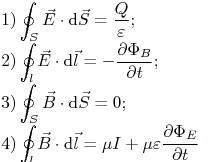
\includegraphics[width=1.0\linewidth]{generalIssues/Figures/maxwell1.png}
		\caption{Postać całkowa.}
		\label{n1}
	\end{subfigure}
	\begin{subfigure}{.49\textwidth}
		\centering
		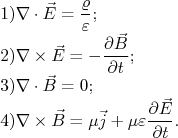
\includegraphics[width=1.0\linewidth]{generalIssues/Figures/maxwell2.png}
		\caption{Postać różniczkowa.}
		\label{r1}
	\end{subfigure}
	\caption{Równania Maxwella.}
	\label{maxwell}
\end{figure}

Rysunek~\ref{maxwell} przedstawia równania Maxwella, gdzie:\newline
$ \varrho $ - gęstość ładunku,\newline
$ \varepsilon $ - przenikalność dielektryczna,\newline
$ \mu $ - przenikalność magnetyczna,\newline
$ \vec{j} $ - gęstość prądu,\newline
$ \Phi_B $- strumień indukcji magnetycznej,\newline
$ \Phi_E $- strumień natężenia pola elektrycznego,\newline
$ \nabla * \vec{F} = \frac{\partial F_x(x,y,z)}{\partial x} + \frac{\partial F_y(x,y,z)}{\partial y} + \frac{\partial F_z(x,y,z)}{\partial z}$ - dywergencja pola wektorowego $ \vec{F} = [F_x, F_y, F_z] $,\newline
$
\nabla \times \vec{F} = 
\begin{vmatrix}
\textbf{i} & \textbf{j} & \textbf{k} \\ 
\frac{\partial}{\partial x} & \frac{\partial}{\partial y} & \frac{\partial}{\partial z} \\ 
F_x & F_y & F_z  \notag
\end{vmatrix}
= (\frac{\partial F_z}{\partial y} - \frac{\partial F_y}{\partial z})\textbf{i} + (\frac{\partial F_x}{\partial z} - \frac{\partial F_z}{\partial x})\textbf{j} + (\frac{\partial F_y}{\partial x} - \frac{\partial F_x}{\partial y})\textbf{k}
$ - rotacja pola wektorowego $ \vec{F} $.\newline

Sens fizyczny praw Maxwella:
\begin{enumerate}[1)]
	\item \underline{Prawo Gaussa dla elektryczności} - źródłem pola elektrycznego są ładunki, a strumień tego pola przez dowolną powierzchnię zamkniętą zależy tylko od ładunku zamkniętego przez tę powierzchnię.
	\item \underline{Prawo Faradaya} - zmiana strumienia indukcji magnetycznej przez powierzchnię zamkniętej pętli powoduje powstanie w tej pętli siły elektromotorycznej indukcji (SEM), a kierunek płynącego prądu jest taki, żeby przeciwdziałać zmianom powodującym indukcję (reguła Lenza).
	\item \underline{Prawo Gaussa dla magnetyzmu} - nie istnieją ładunki magnetyczne, a strumień pola magnetycznego przez dowolną powierzchnię zamkniętą jest równy 0.
	\item \underline{Prawo Ampere'a} - zmienne pole elektryczne i płynący prąd powodują powstanie pola magnetycznego.
\end{enumerate}

Dla fali elektromagnetycznej w próżni wektory $ \vec{E} $ i $ \vec{B} $ drgają w płaszczyznach wzajemnie prostopadłych i dla fali rozchodzącej się w kierunku osi x możemy przyjąć taki układ odniesienia aby wektor $ \vec{E} $ drgał w kierunku osi y a wektor $ \vec{B} $ w kierunku osi z. Zatem wektory $ \vec{E} $ i $ \vec{B} $ mają tylko po jednej składowej:\newline
$ \vec{E} = [0, E, 0] $,\newline
$ \vec{B} = [0, 0, B] $.\newline
Liczmy rotację wektorów $ \vec{E} $ i $ \vec{B} $ (wykorzystując fakt, że nasza fala jest falą płaską i pola $ \vec{E} $ i $ \vec{B} $ zmieniają się tylko względem współrzędnej x, czyli że $ \frac{\partial E}{\partial z} = 0, \frac{\partial B}{\partial y} = 0$):\newline
$ \nabla \times \vec{E} = \textbf{k}\frac{\partial E}{\partial x} $,\newline
$ \nabla \times \vec{B} = -\textbf{j}\frac{\partial B}{\partial x} $.\newline

Korzystając z równań Faradaya oraz Ampera w postaci różniczkowej otrzymujemy (poszukujemy równania dla fal elektromagnetycznych rozchodzących się w próżni gdzie nie będą występowały prądy przewodzenia, czyli $ \vec{j} $ = 0):\newline
$ \textbf{k}\frac{\partial E}{\partial x} = -\frac{\partial \vec{B}}{\partial t} = -\textbf{k}\frac{\partial B}{\partial t} $,\newline
$ \textbf{j}\frac{\partial B}{\partial x} = -\mu_0 \epsilon_0 \frac{\partial \vec{E}}{\partial t} = -\textbf{j} \mu_0 \epsilon_0 \frac{\partial E}{\partial t} $.\newline
W efekcie dostajemy układ dwóch równań:\newline
$ \frac{\partial E}{\partial x} = -\frac{\partial B}{\partial t} $,\newline
$ \frac{\partial B}{\partial x} = - \mu_0 \epsilon_0 \frac{\partial E}{\partial t} $.\newline

Równania falowe dla $ \vec{E} $ i $ \vec{B} $ będą miały identyczną postać. Jeżeli zdecydujemy się szukać równania dla $ \vec{E} $, to eliminujemy z naszego układu równań $ \vec{B} $ przez utworzenie pochodnych mieszanych $ \vec{E} $ względem x i t. Różniczkujemy zatem pierwsze równanie po x, a drugie po t (jeśli chcemy szukać równania dla $ \vec{B} $ eliminujemy w ten sam sposób z naszych równań $ \vec{E} $):\newline
$ \frac{\partial^2 E}{\partial x^2} = -\frac{\partial^2 B}{\partial t \partial x} $,\newline
$ \frac{\partial^2 B}{\partial t \partial x} = - \mu_0 \epsilon_0 \frac{\partial^2 E}{\partial t^2} $.\newline
Z powyższego układu równań otrzymujemy poszukiwane równanie falowe dla pola $ \vec{E} $:\newline
$ \frac{\partial^2 E}{\partial x^2} - \mu_0 \epsilon_0 \frac{\partial^2 E}{\partial t^2} = 0 $\newline
Znając ogólną postać równania falowego dla fali rozchodzącej się z predkością v w kierunku osi x:\newline
$ \frac{\partial^2 \xi}{\partial x^2} - \frac{1}{v^2} \frac{\partial^2 \xi}{\partial t^2} = 0 $\newline
otrzymujemy związek pomiędzy prędkością światła w próżni (c) a wartościami przenikalności elektrycznej i magnetycznej próżni: \newline
$ c = \frac{1}{\sqrt{\mu_0 \epsilon_0}} $.\newline
Rozwiązanie równania falowego dla pola $ \vec{E} $ ma postać:\newline
$ \vec{E} = \vec{E_0}\sin(kx - \omega t) $,\newline
gdzie: $ k = \frac{2\pi}{\lambda} $, $ \omega = ck $.
	
	\subsection{Właściwości fal elektromagnetycznych.}
	Falą elektromagnetyczną nazywamy rozchodzące się w przestrzeni zaburzenie pola elektromagnetycznego. Składowa elektryczna i magnetyczna fali indukują się wzajemnie – zmieniające się pole elektryczne wytwarza zmieniające się pole magnetyczne, a z kolei zmieniające się pole magnetyczne wytwarza zmienne pole elektryczne.

Promieniowanie elektromagnetyczne przejawia właściwości falowe ulegając interferencji, dyfrakcji, spełnia prawo odbicia i załamania. W wyniku superpozycji fal elektromagnetycznych może powstać fala stojąca. 

Strumień energii przenoszonej przez falę elektromagnetyczną w każdym punkcie przestrzeni określa wektor Poyntinga zdefiniowany jako:\newline
$ \vec{S} = \frac{1}{\mu_0} \vec{E} \times \vec{B} $,\newline
gdzie:\newline
$ \mu_0 $ - przenikalność magnetyczna próżni,\newline
$ \vec{E} $ - natężenie pola elektrycznego,\newline
$ \vec{B} $ - indukcja pola magnetycznego.

Choć w elektrodynamice klasycznej energię promieniowania elektromagnetycznego uważa się za wielkość ciągłą, zależną jedynie od natężenia pola elektrycznego i indukcji pola magnetycznego, to zjawiska zachodzące na poziomie atomowym dowodzą, że jest ona skwantowana. Energia pojedynczego kwantu jest zależna tylko od częstotliwości fali $ \nu $ i wynosi:\newline
$ E = h \nu $, gdzie \textit{h} - stała Plancka.

Właściwości fal elektromagnetycznych zależą od długości fali. Promieniowaniem elektromagnetycznym o różnej długości fali są:
 
\begin{enumerate}[-]
	\item \underline{Fale radiowe} (długość fali powyżej 1 m) - znajdują bardzo szerokie zastosowanie w telekomunikacji, radiofonii, telewizji, radioastronomii i wielu innych dziedzinach nauki i techniki. Naturalne źródła fal radiowych to między innymi wyładowania atmosferyczne, zorze polarne, radiogalaktyki.
	\item \underline{Mikrofale} (od 1 mm do 1 m) - podstawowe zastosowania mikrofal to łączność (na przykład telefonia komórkowa, radiolinie, bezprzewodowe sieci komputerowe) oraz technika radarowa. Fale zakresu mikrofalowego są również wykorzystywane w radioastronomii, a odkrycie mikrofalowego promieniowania tła miało ważne znaczenie dla rozwoju i weryfikacji modeli kosmologicznych. Wiele dielektryków mocno absorbuje mikrofale, co powoduje ich rozgrzewanie i jest wykorzystywane w kuchenkach mikrofalowych, przemysłowych urządzeniach grzejnych i w medycynie.
	\item \underline{Podczerwień} (od 700 nm do 1 mm) - promieniowanie podczerwone jest nazywane również cieplnym, szczególnie gdy jego źródłem są nagrzane ciała. Każde ciało o temperaturze większej od zera bezwzględnego emituje takie promieniowanie, a ciała o temperaturze pokojowej najwięcej promieniowania emitują w zakresie długości fali rzędu 10 $ \mu m $. Przedmioty o wyższej temperaturze emitują promieniowanie o większym natężeniu i mniejszej długości, co pozwala na zdalny pomiar ich temperatury i obserwację za pomocą urządzeń rejestrujących wysyłane promieniowanie (termowizja).
	\item \underline{Światło widzialne} (od 380 nm do 700 nm) - światło (promieniowanie widzialne) to ta część widma promieniowania elektromagnetycznego, na którą reaguje zmysł wzroku człowieka. Różne zwierzęta mogą widzieć w nieco różnych zakresach. Światło ma bardzo duże znaczenie w nauce i wiele zastosowań w technice. Dziedziny nauki i techniki zajmujące się światłem noszą nazwę optyki.
	\item \underline{Ultrafiolet} (od 10 nm do 380 nm) - promieniowanie ultrafioletowe jest zaliczane do promieniowania jonizującego, czyli ma zdolność odrywania elektronów od atomów i cząsteczek. W technice ultrafiolet stosowany jest powszechnie. Powoduje świecenie (fluorescencję) wielu substancji chemicznych. W świetlówkach ultrafiolet wytworzony na skutek wyładowania jarzeniowego pobudza luminofor do świecenia w zakresie widzialnym. Niektóre owady, na przykład pszczoły, widzą w bliskiej światłu widzialnemu części widma promieniowania ultrafioletowego, również rośliny posiadają receptory ultrafioletu. 
	\item \underline{Promieniowanie rentgenowskie} (od 5 pm do 10 nm) - promieniowanie rentgenowskie jest promieniowaniem jonizującym. Technicznie promieniowanie rentgenowskie uzyskuje się przeważnie poprzez wyhamowywanie rozpędzonych cząstek naładowanych. W lampach rentgenowskich są to rozpędzone za pomocą wysokiego napięcia elektrony hamowane na metalowych anodach. Źródłem wysokoenergetycznego promieniowania rentgenowskiego są również przyspieszane w akceleratorach cząstki naładowane. Promieniowanie rentgenowskie jest wykorzystywane do wykonywania zdjęć rentgenowskich do celów defektoskopii i diagnostyki medycznej. W zakresie promieniowania rentgenowskiego są również prowadzone obserwacje astronomiczne. 
	\item \underline{Promieniowanie gamma} (0,03 pm do 300 pm) - promieniowania gamma jest promieniowaniem jonizującym. Promieniowanie gamma towarzyszy reakcjom jądrowym, powstaje w wyniku anihilacji – zderzenie cząstki i antycząstki, oraz rozpadów cząstek elementarnych. Otrzymywane w cyklotronach promieniowanie hamowania i synchrotronowe również leży w zakresie długości fali promieniowania gamma, choć niekiedy bywa nazywane wysokoenergetycznym promieniowaniem rentgenowskim. Promienie gamma mogą służyć do sterylizacji żywności i sprzętu medycznego. W medycynie używa się ich w radioterapii oraz w diagnostyce. Zastosowanie w przemyśle obejmują badania defektoskopowe. Astronomia promieniowania gamma zajmuje się obserwacjami w tym zakresie długości fal. 
\end{enumerate}
	
	\subsection{Interferencja i dyfrakcja fal.}
	\underline{Interferencja} jest to zjawisko powstawania nowego, przestrzennego rozkładu amplitudy fali (wzmocnienia i wygaszenia) w wyniku nakładania się (superpozycji fal) dwóch lub więcej fal. Warunkiem trwałej interferencji fal jest ich spójność, czyli korelacja faz i równość częstotliwości. 

Dla najprostszego przypadku dwóch fal harmonicznych o jednakowych amplitudach A, jednakowej długości fali $ \lambda $ i zgodnych fazach początkowych, rozchodzących się z dwóch różnych źródeł, które leżą w odległościach odpowiednio $ d_1 $ i $ d_2 $ od punktu P, zaburzenie w punkcie P opisuje wzór:\newline
$ y(P) = A\sin (\omega t + \phi_1) + A\sin (\omega t + \phi_2)$, gdzie:\newline
$ \phi_1 = 2\pi\frac{d_1}{\lambda} $,\newline
$ \phi_2 = 2\pi\frac{d_2}{\lambda} $.\newline
Gdy spełniony jest warunek:\newline
$ \phi_1 - \phi_2 = 2\pi\frac{d_1-d_2}{\lambda} = 2k\pi $,\newline
gdzie k - dowolna liczba naturalna, to fale w punkcie P ulegają wzmocnieniu (są w tej samej fazie) i:\newline
$ y(P) = 2A\sin (\omega t) $.\newline
Gdy natomiast w pewnym punkcie $ P_1 $:\newline
$ \phi_1 - \phi_2 = 2\pi\frac{d_1-d_2}{\lambda} = (2k+1)\pi $\newline
wtedy fale wygaszają się (są w przeciwfazie) i:\newline
$ y(P_1) = 0 $.

Interferencja pozwala na bardzo precyzyjny pomiar zmian długości drogi od źródła do detektora fali.

\underline{Dyfrakcja} (ugięcie fali) – zespół zjawisk związanych ze zmianą kierunku rozchodzenia się fali będący odstępstwem od praw optyki geometrycznej (dział optyki zajmujący się wytłumaczeniem zjawisk optycznych przy użyciu pojęcia promienia). Dyfrakcję w węższym znaczeniu określa się jako ugięcie światła wokół krawędzi przeszkody lub otworu w obszarze cienia przeszkody.

Zjawisko dyfrakcji rozpatruje się jako interferencję fal cząstkowych powstających zgodnie z zasadą Huygensa. Jest to zasada stosowana do określenia rozchodzenia się fali w ośrodku, mówiąca, iż każdy punkt ośrodka, do którego dotarło czoło fali, można uważać za źródło nowej fali kulistej. Wypadkową powierzchnię falową tworzy powierzchnia styczna do wszystkich powierzchni fal cząstkowych i ją właśnie obserwuje się w ośrodku.

Rysunek~\ref{diffracion} przedstawia dyfrakcję na pojedynczej szczelinie. Gdy różnica dróg fali ze skrajnego i środkowego elementu równa jest połowie długości fali, to fale z obu połówek szczeliny wygaszą się. Jeżeli wiązki są niemal równoległe, to różnica odległości pojawia się tylko przy wyjściu promieni ze szczeliny, wówczas:\newline
$ d\sin(\theta_{min}) = \lambda $.\newline

Przepuszczenie fali przez szczelinę dyfrakcyjną pozwala na określenie kierunku rozchodzenia się fali. Im mniejsza jest szerokość szczeliny, tym dokładniej można to zrobić. Jednocześnie zmniejszanie szczeliny powoduje, że trudniej jest określić energię fali, ponieważ rozprasza się ona na większy obszar. W efekcie iloczyn błędu określenia energii oraz błędu pomiaru kierunku musi być większy od pewnej stałej. Oznacza to, że istnieje granica dokładności pomiaru parametrów rozchodzącej się fali. Próba dokładniejszego określenia jednego z parametrów fali powoduje zwiększenie niepewności pomiaru drugiego sprzężonego z nim. Zjawisko to ma fundamentalne znaczenie, jeżeli weźmie się pod uwagę, że każda materialna cząstka jest falą. Zjawisko to w mechanice kwantowej odpowiada zasadzie nieoznaczoności

\begin{figure} [H]
	\centering
	\begin{subfigure}{.99\textwidth}
		\centering
		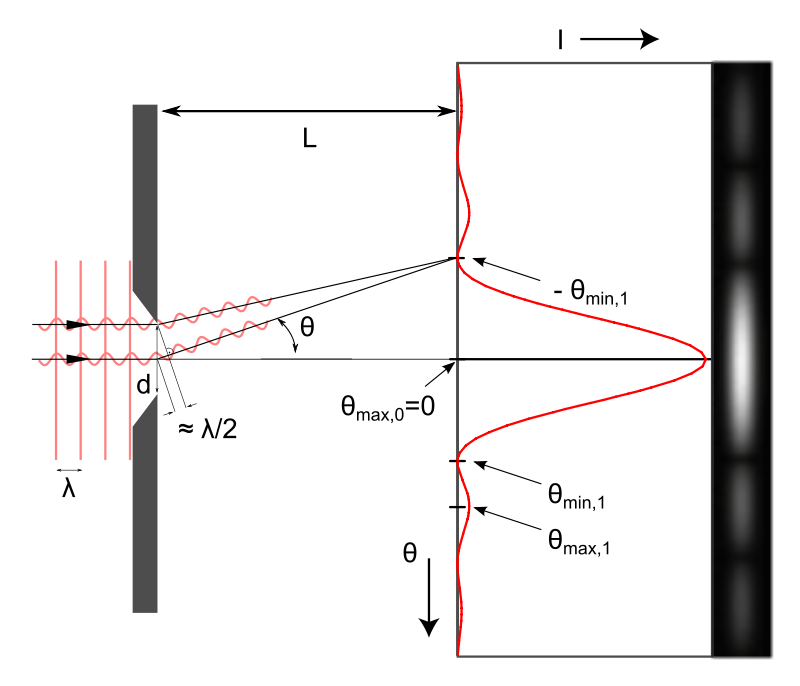
\includegraphics[width=0.6\linewidth]{generalIssues/Figures/diffraction.png}
	\end{subfigure}
	\caption{Dyfrakcja na pojedynczej szczelinie.}
	\label{diffracion}
\end{figure}

Pierwszą najprostszą formę eksperymentu przejścia światła przez podwójną szczelinę (rysunek~\ref{diffracion2}), zwaną obecnie doświadczenie Younga wykonał Thomas Young w 1801 roku. Eksperyment ten był zaczątkiem do uznania w XIX w falowej teorii światła. 

\begin{figure} [H]
	\centering
	\begin{subfigure}{.99\textwidth}
		\centering
		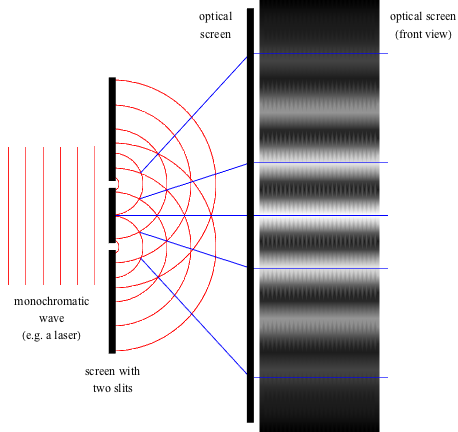
\includegraphics[width=0.6\linewidth]{generalIssues/Figures/diffraction2.png}
	\end{subfigure}
	\caption{Przejście światła przez podwójną szczelinę.}
	\label{diffracion2}
\end{figure}

Dla obrazów dyfrakcyjnych powstałych po przejściu światła przez otwór kołowy definiuje się \underline{warunek Rayleigha} określający zdolność rozdzielczą elementów i układów optycznych:\newline
$ \phi \approx \sin(\phi) = 1.22 \frac{\lambda}{d} $ (przybliżenie dla małych kątów), gdzie:\newline
$ \phi $ - minimalny kąt między promieniami, których obrazy mają być rozróżnialne, czyli inaczej – ich odległość kątowa,\newline
$ \lambda $ - długość fali światła,\newline
$ d $ - średnica otworu.\newline

Aby wzmocnić falę przechodzącą przez szczelinę stosuje się w optyce układy wielu takich szczelin, nazywane \underline{siatką dyfrakcyjną} (rysunek~\ref{diffracion3}). Efekty optyczne od każdej szczeliny dodają się, przez co zachowanie fali zależy tylko od stałej siatki (odległości dzielącej najbliższe sobie rysy). Zjawisko dyfrakcji zachodzi również, kiedy fale przechodzą przez wiele blisko siebie położonych warstw. Jeżeli odległość między warstwami jest stała, kolejne maksima fali można opisać zależnością:\newline
$ \sin(\theta) = \frac{n\lambda}{d} $, gdzie:\newline
$ d $ - stała siatki,\newline
$ \theta $ - kąt od osi wiązki światła,\newline
$ \lambda $ - długość fali,\newline
$ d $ - przyjmuje wartości całkowite dodatnie od 1,2,3,...\newline

\begin{figure} [H]
	\centering
	\begin{subfigure}{.99\textwidth}
		\centering
		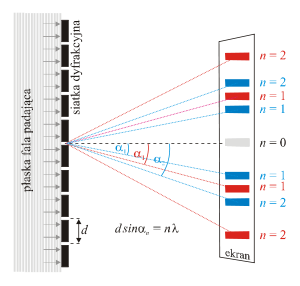
\includegraphics[width=0.6\linewidth]{generalIssues/Figures/diffraction3.png}
	\end{subfigure}
	\caption{Siatka dyfrakcyjna.}
	\label{diffracion3}
\end{figure}

Zjawisko dyfrakcji pozwoliło na rozwój krystalografii rentgenowskiej, dzięki której badano strukturę kryształów, odkryto w ten sposób także strukturę spirali DNA. 
	
	\subsection{Zasady termodynamiki.}
	\underline{Zerowa zasada termodynamiki} - jeśli układy A i B mogące ze sobą wymieniać ciepło si ą ze sobą w równowadze termicznej, i to samo jest prawdą dla układów B i C, to układy A i C również są ze sobą w równowadze termicznej. Z zasady tej wynika istnienie temperatury empirycznej. Temperatura to taka wielkość fizyczna, która dla układów A, B i C jest równa, gdy ustaje przepływ ciepła. Układy będą ze sobą w równowadze termodynamicznej. Zerowa zasada termodynamiki stwierdza także, że ciało w równowadze termodynamicznej ma wszędzie tę samą temperaturę.

\underline{Pierwsza zasada termodynamiki} - zmiana energii wewnętrznej (będącej funkcją stanu) układu zamkniętego (nie wymienia masy z otoczeniem) jest równa energii, która przepływa przez jego granice na sposób ciepła i pracy:\newline
$ \Delta U = W + Q $, gdzie:\newline
$ \Delta U $ - zmiana energii wewnętrznej układu,\newline
$ W $ - praca wykonana na układzie,\newline
$ Q $ - ciepło przekazane do układu.\newline
Alternatywne sformułowanie - nie istnieje perpetuum mobile pierwszego rodzaju (maszyna, która wytwarza więcej energii, niż sama zużywa).

\underline{Druga zasada termodynamiki} - w układzie termodynamicznie izolowanym istnieje funkcja stanu zwana entropią, która nie maleje z czasem. Matematyczny zapis tego faktu to następujące sformułowanie: zmiana entropii $ \Delta S $ w dowolnym procesie odwracalnym jest równa całce z przekazu ciepła DQ podzielonego przez temperaturę T. W procesie nieodwracalnym natomiast zmiana entropii jest większa od tej całki:
$ \Delta S \geq \int \frac{DQ}{T} $\newline
Różnica ta jest miarą nieodwracalności procesu i jest związana z rozpraszaniem energii. Entropia (S) jest funkcją stanu będąca miarą liczby sposobów (W), na jakie może być zrealizowany określony stan termodynamiczny danego układu w określonej temperaturze (T). Układ dąży do stanu, który może być w danych warunkach zrealizowany na jak najwięcej sposobów; dąży więc on do maksymalizacji entropii. Nie można bez wkładu pracy przesyłać energii termicznej między ciałami mającymi tę samą temperaturę. Oznacza to, że perpetuum mobile drugiego rodzaju (maszyna, która zamienia energię cieplną na pracę mechaniczną bez wzrostu całkowitej entropii) nie istnieje. 

\underline{Trzecia zasada termodynamiki} - nie można za pomocą skończonej liczby kroków uzyskać temperatury zera bezwzględnego (zero kelwinów), jeżeli za punkt wyjścia obierzemy niezerową temperaturę bezwzględną. Podstawą takiego zdefiniowania III zasady termodynamiki jest analiza sprawności lodówki. Jak wiemy, lodówka działa na zasadzie odwrotnego cyklu Carnota, a jej sprawność dana jest wzorem:\newline
$ n = \frac{Q_{odebrane}}{W} = \frac{T_2}{T_1-T_2} $\newline
Jeżeli ciało o określonej temperaturze $ T_1 $ chcielibyśmy schłodzić do $ T_2 \to $, odbierając przy tym skończone ciepło $ Q $, to analizując wzór widzimy, że w takim wypadku $ \frac{Q}{W} \to 0 $, czyli $ W\to $ nieskończoności. Gdybyśmy podstawili $ T_2 = 0 $, równanie nie miałoby sensu matematycznego, co oznacza, że nie da się osiągnąć temperatury zera bezwzględnego w skończonej liczbie kroków. Mówiąc inaczej, gdyby udało się schłodzić jakąś substancję do 0 K i gdyby utworzyła ona kryształ doskonały nieposiadający zamrożonych defektów krystalicznych, to jej entropia musiałaby przyjąć wartość 0. Jest to jednak technicznie, a także formalnie, niewykonalne:
$ \lim_{T\to0} S = 0 $
	
	\subsection{Entropia w ujęciu termodynamicznym i statystycznym.}
	Entropia jest to termodynamiczna funkcja stanu, określająca kierunek przebiegu procesów spontanicznych (samorzutnych) w odosobnionym układzie termodynamicznym. Entropia jest miarą stopnia nieuporządkowania układu i rozproszenia energii. Jest wielkością ekstensywną. Zgodnie z drugą zasadą termodynamiki, jeżeli układ termodynamiczny przechodzi od jednego stanu równowagi do drugiego, bez udziału czynników zewnętrznych (a więc spontanicznie), to jego entropia zawsze rośnie. W ramach II zasady termodynamiki zmiana entropii (w procesach kwazistatycznych) jest zdefiniowana przez swoją różniczkę zupełną jako:\newline
$ dS = \frac{1}{T}\delta Q $, gdzie:\newline
$ T $ - temperatura bezwzględna,\newline
$ \delta Q $ - ciepło elementarne, czyli niewielka ilość ciepła dostarczonego do układu.\newline
Entropię pewnego stanu termodynamicznego P można wyznaczyć ze wzoru:\newline
$ S(P) = \int_{0}^{T_p}\frac{C(T)dT}{T} $, gdzie:\newline
$ C(T) $ - pojemność cieplna (ilość ciepła, jaka jest niezbędna do zmiany temperatury ciała o jednostkę temperatury),\newline
$ T_p $ - temperatura w stanie P.
Podstawowe równanie termodynamiki fenomenologicznej, w którym występuje entropia, ma postać:\newline
$ dU = TdS - pdV + \sum_{i=1}^{k}\mu_idN_i $, gdzie:\newline
$ U $ - energia wewnętrzna,\newline
$ k $ - liczba różnych składników,\newline
$ T $ - temperatura,\newline
$ p $ - ciśnienie,\newline
$ \mu_i $ - potencjał chemiczny i-tego składnika.

W termodynamice statystycznej całkowita entropia układu makroskopowego jest równa:\newline
$ S = k\ln(W) $\newline
lub\newline
$ S = -k\sum_{i}p_i\ln(p_i) $, gdzie:\newline
$ k $ - stała Boltzmanna,\newline
$ W $ - liczba sposobów, na jakie makroskopowy stan termodynamiczny układu (makrostan) może być zrealizowany poprzez stany mikroskopowe (mikrostany),\newline
$ p_i $ - prawdopodobieństwo i-tego mikrostanu.\newline
Zatem $ \log_2(W) $ jest liczbą bitów potrzebnych do określenia, którą realizację przyjął dany układ.


	
	\subsection{Klasyczne i kwantowe rozkłady statystyczne.}
	\underline{Gaz doskonały} - zwany też gazem idealnym, jest to abstrakcyjny, matematyczny model fizyczny gazu, spełniający następujące warunki: 

\begin{enumerate}[-]
	\item brak oddziaływań miedzycząsteczkowych z wyjątkiem odpychania w momencie zderzeń cząsteczek,
	\item objętość cząsteczek jest znikoma w stosunku do objętości gazu.
	\item zderzenia cząsteczek są doskonale sprężyste,
	\item cząsteczki znajdują się w ciągłym, chaotycznym ruchu.
\end{enumerate}

\underline{Rozkład Maxwella} – wzór określający rozkład prędkości cząstek gazu doskonałego. Założenie:  funkcja rozkładu f zależy tylko od wartości prędkości v:\newline
$ f(v_x,v_y,v_z) = f(v_x^2+v_y^2+v_z^2) $\newline
Żaden kierunek nie jest uprzywilejowany, ruch w każdym z kierunków x,y i z odbywa się niezależnie:\newline
$ f(v_x,v_y,v_z) = h(v_x)h(v_y)h(v_z) $\newline
Funkcja rozkładu h jest taka sama dla każdego kierunku co wynika z symetrii.\newline
$ ln[h(v_x)] + ln[h(v_y)] + ln[h(v_z)] = ln[f(v_x^2+v_y^2+v_z^2)] $, stąd:\newline
$ h(v_x) = C_xe^{(-Bv_x^2)} $\newline
$ f(v) = C_xC_yC_ze^{-B(v_x^2+v_y^2+v_z^2)} = Ce^{-Bv^2} $\newline
Stałą C znajdziemy z warunku normalizacji natomiast stałą B znajdujemy na podstawie równania łączącego średni kwadrat prędkości cząsteczek z temperaturą oraz wyrazić wartość średnią kwadratu prędkości poprzez funkcję gęstości prawdopodobieństwa:\newline
$ \frac{m<v^2>}{2} = \frac{3}{2}kT = \frac{m}{2}\int_{0}^{\infty} v^2f(v)*4\pi v^2dv $, gdzie:
$ m $ - masa cząsteczki,\newline
$ k $ - stała Boltzmanna,\newline
$ 4\pi v^2dv $ - element objętości przestrzeni prędkości (v, v+dv) we współrzędnych sferycznych.\newline
Otrzymujemy ostatecznie:\newline
$ f(v) = (\frac{m}{2\pi kT})^{\frac{3}{2}}e^{\frac{mv^2}{2kT}} $\newline
$ \frac{dP}{dv} = 4\pi (\frac{m}{2\pi kT})^{\frac{3}{2}}v^2e^{\frac{mv^2}{2kT}} $ - gęstość prawdopodobieństwa wystąpienia cząsteczki o prędkości v.\newline
Rozkład Maxwella pokazuje, że prędkości cząsteczek zależą od temperatury oraz masy molowej. Wraz ze wzrostem temperatury rozkład się poszerza (rysunek~\ref{maxwellDistribution}), a jego prędkość najbardziej prawdopodobna (tam gdzie dP/dv jest największe), jak i średnia prędkość (<v>) oraz średnia prędkość kwadratowa ($ \sqrt{<v^2>} $) zwiększają się.

\begin{figure} [H]
	\centering
	\begin{subfigure}{1.0\textwidth}
		\centering
		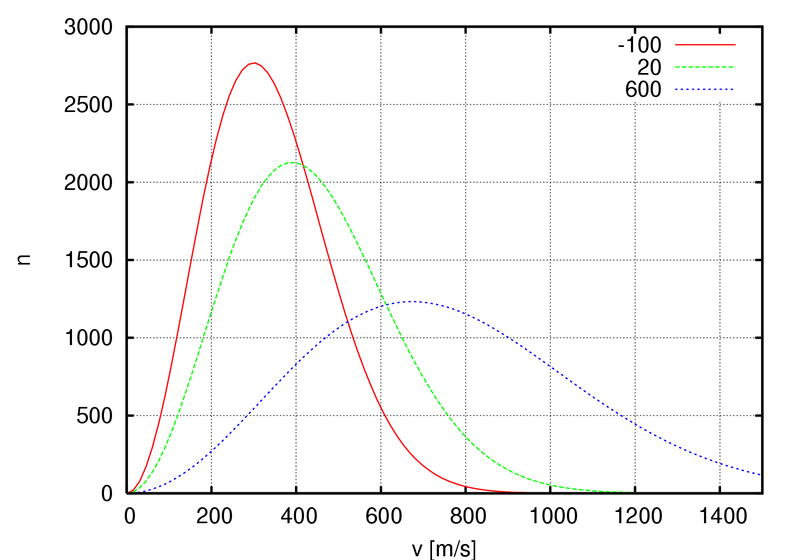
\includegraphics[width=0.98\linewidth]{generalIssues/Figures/maxwellDistribution.png}
	\end{subfigure}
	\caption{Rozkład Maxwella dla tlenu dla trzech temperatur (–100 $ ^\circ C $, temperatura pokojowa i 600 $ ^\circ C $). Wartość funkcji odpowiada liczbie cząsteczek spośród 1 miliona cząsteczek, jaka będzie poruszać się z prędkością v+/-0,5 m/s.}
	\label{maxwellDistribution}
\end{figure}

Wzór na koncentrację cząsteczek, czyli ich liczbę w jednostce objętości:\newline
$ n = n_0\exp(-\frac{E_p}{kT}) $, gdzie:\newline
$ E_p $ - energia potencjalna cząstek w danym stanie (np. na danej wysokości),\newline
$ n_0 $ - koncentracja cząsteczek dla $ E_p = 0 $ (np. koncentracja na powierzchni ziemi).\newline

Wzór ten wyraża zależność koncentracji cząsteczek od ich wysokości lub energii potencjalnej. Wynikający z niego rozkład koncentracji nosi nazwę rozkładu Boltzmanna i odnosi się nie tylko do pola sił przyciągania ziemskiego, ale do dowolnego pola potencjalnego, jeśli tylko cząsteczki poruszają się chaotycznym ruchem cieplnym. Liczba cząsteczek w objętości $ dV = dz \cdot dy \cdot dz $, której położenie określają współrzędne $ (x,y,z) $ wynosi:\newline
$ dn(x,y,z) = n_0\exp(-\frac{E_p(x,y,z)}{kT})dx\cdot dy\cdot dz $\newline
Nietrudno tu zauważyć podobieństwo rozkładów Maxwella i Boltzmanna, z tą różnicą, że pierwszy wyraża zależność od kwadratu prędkości lub energii kinetycznej, drugi - od energii potencjalnej. Rozkład zawierający obie te zależności nosi nazwę rozkładu Maxwella-Boltzmanna i ma postać:
$ dn(x,y,z,v_x,v_y,v_z) = A\exp(-\frac{E_p+E_k}{kt})dx\cdot dy \cdot dz \cdot v_x \cdot v_y \cdot v_z $

\underline{Zakaz Pauliego} głosi, że prawdopodobieństwo znalezienia w układzie fermionów (cząstek o spinie połówkowym) pary cząstek o jednakowych liczbach kwantowych jest równe zeru (czyli np. możemy znaleść na tej samej orbicie atomowej dwa elektrony, ale muszą mieć przeciwne spiny - jest to przykład degeneracji).

Zgodnie z rozkładem Fermiego-Diraca (rysunek~\ref{fermi})średnia liczba cząstek w niezdegenerowanym stanie energetycznym $ E $ dana jest przez:\newline

$ <n> = \dfrac{1}{e^{\beta (E-\mu)}+1} $, gdzie:\newline
$ E $ - energia tego stanu,\newline
$ \mu $ - potencjał chemiczny,\newline
$ \beta = 1/k_bT $\newline

\begin{figure} [H]
	\centering
	\begin{subfigure}{1.0\textwidth}
		\centering
		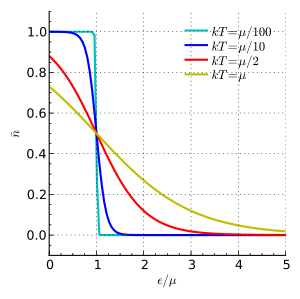
\includegraphics[width=0.7\linewidth]{generalIssues/Figures/fermi.png}
	\end{subfigure}
	\caption{Rozkład Fermiego-Diraca. Oś pozioma: $ E/\mu $. Oś pionowa: $ <n> $.}
	\label{fermi}
\end{figure}

W temperaturze zera bezwzględnego wprowadza się oznaczenie $ \mu = \mu(0) = E_F $ - jest to energia najwyżej obsadzonego stanu ($ k_F $ - poziom Fermiego) w temperaturze zera bezwzględnego. W tej temperaturze obsadzone są wszystkie stany o energii mniejszej lub równej energii Fermiego ($ E_F $ a wyższe stany nie są obsadzone.Dla każdej temperatury $ T $ zachodzi $ P(E_k) = 0.5 $ gdy $ E_k = \mu $. Dla takich energii, że $ E_k - \mu \gg k_BT $ rozkład przechodzi w klasyczny rozkład Boltzmanna.

Statystyka Bosego-Einsteina dotyczy bozonów (cząstek o spinie całkowitym, których nie obowiązuje zakaz Pauliego) traktowanych jako gaz bozonowy. Zgodnie z rozkładem Bosego-Einsteina średnia liczba cząstek w danym stanie kwantowym jest równa:

$ <n_i> = \dfrac{n}{Z}\dfrac{g_i}{e^{\beta(E_i-\mu)}-1} $, gdzie:\newline
$ E_i $ - energia i-tego stanu,\newline
$ g_i $ - degeneracja i-tego stanu,\newline
$ n $ - całkowita liczba cząstek,\newline
$ \mu $ - potencjał chemiczny,\newline
$ Z = \sum_{i}\dfrac{g_i}{e^{\beta(E_i-\mu)}-1} $ - suma statystyczna.\newline
Potencjał chemiczny w tym rozkładzie jest zawsze ujemny lub równy zeru. Gdy temperatura jest wysoka, można zaniedbać składnik –1 i rozkład przechodzi w rozkład fizyki klasycznej - klasyczny rozkład Boltzmanna. Rozkładowi Bosego-Einsteina podlegają fotony (o spinie 1) – nosi on wtedy nazwę rozkładu Plancka, który tłumaczy promieniowanie ciała doskonale czarnego. Jego wprowadzenie przez Plancka zapoczątkowało mechanikę kwantową. Zakaz Pauliego nie dotyczy bozonów, umożliwia to ich kondensację.
\underline{Kondensacja Bosego-Einsteina} – efekt kwantowy zachodzący w układach podległych rozkładowi Bosego-Einsteina. W temperaturach niższych od temperatury krytycznej część cząstek (bozonów) przechodzi w zerowy stan pędowy – cząstki te mają identyczny pęd. Oznacza to, że w zerowej objętości przestrzeni pędów może znajdować się niezerowa liczba cząstek. Mówi się wtedy o makroskopowym obsadzeniu stanu podstawowego. Efektem kondensacji jest kolektywne zachowanie wszystkich cząstek biorących w niej udział (w przybliżeniu wszystkie zachowują się jak jedna cząstka). Nie chodzi tu o kondensację w zwykłym sensie w przestrzeni położeniowej – cząstki nie znajdują się w jednym miejscu, lecz o "kondensację" cząstek w przestrzeni pędów – znaczna liczba cząstek ma taki sam pęd. Rozkład przestrzenny cząstek "skondensowanych" pozostaje równomierny (jeśli nie ma pól zewnętrznych). W kondensacie Bosego-Einsteina zachodzi zjawisko nadciekłości. 

	
	\subsection{Budowa materii.}
	Model standardowy – teoria fizyki cząstek podstawowych, zwanych też cząstkami elementarnymi, które są podstawowymi składnikami każdej materii (rys.~\ref{standard_model}). Opisuje trzy z czterech (z wyjątkiem grawitacji) oddziaływań podstawowych: elektromagnetyczne, słabe i silne. Sformułowana jest w języku matematyki, opisując relacjami matematycznymi zależności między elementami tej teorii. Opiera się na koncepcji pola Yanga-Millsa (pole rządzące oddziaływaniem wszystkich znanych cząstek we wszechświecie).

\begin{figure} [H]
	\centering
	\begin{subfigure}{.99\textwidth}
		\centering
		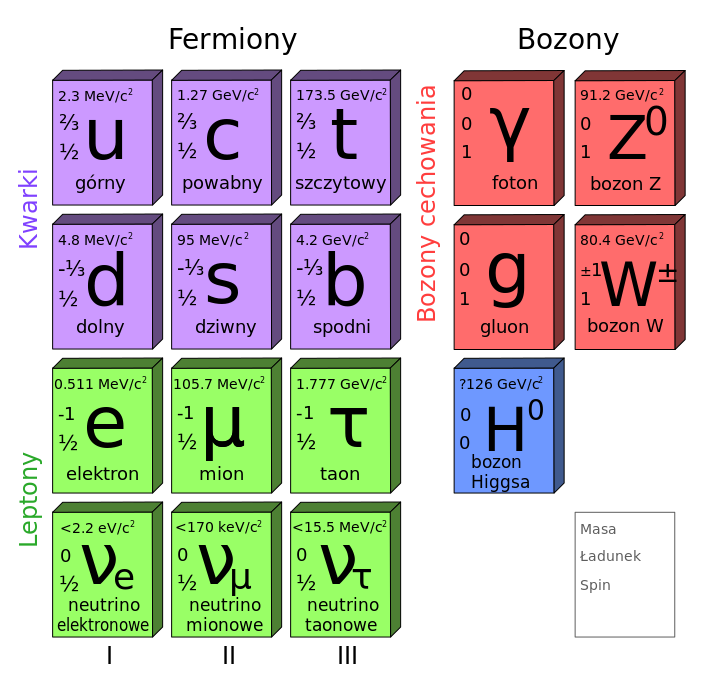
\includegraphics[width=0.7\linewidth]{generalIssues/Figures/standard_model.png}
	\end{subfigure}
	\caption{Cząstki elementarne według Modelu Standardowego.}
	\label{standard_model}
\end{figure}

Fermiony są podstawowymi elementami budującymi materię. Materię trwałą, która nas otacza, tworzą następujące cząstki: elektron, kwark górny (u) oraz kwark dolny (d) np.  dwa kwarki górne i jeden dolny (uud) tworzą proton. Kwarki mają kolor i zapach (są to nazwy nadane umownie pewnym liczbom kwantowym). Do tej grupy cząstek należy też neutrino elektronowe, a grupa ta tworzy pierwszą generację. Kolejne dwie generacje zawieraja po cztery cząstki odpowiadające cząstkom z pierwszej generacji (lecz o różnej masie).

Bozony cechowania przenoszą oddziaływania:
\begin{itemize}
	\item elektromagnetyczne - przenoszone jest przez foton. Oddziaływanie to odbywa się poprzez wytworzenie lub pochłonięcie fotonu.
	\item słabe - powodujące między innymi rozpady beta, przenoszone jest przez bozony $ W^+ $ i $ W^- $ oraz $ Z^0 $.
	\item silne - łączące kwarki w hadrony, przenoszone jest przez osiem rodzajów gluonów, sposób oddziaływania (rodzaj gluonu) oznaczany jest właściwością nazywaną kolorem gluonu. Hadrony złożone są z kwarków występujących przeważnie trójkami (trzy kwarki lub trzy antykwarki tworzą bariony - spin połówkowy, liczba barionowa = 1) lub parami (pary kwark i antykwark tworzą mezony - spin całkowity, liczba barionowa = 0). Właściwością hadronów jest również ich całkowity ładunek elektryczny.
\end{itemize}

Bozon Higgsa (istnienie którego udało się potwierdzić doświadczalnie w 2012 roku) oddziałując z innymi cząstkami nadaje im masę (głównie dotyczy nadawania masy elektronowi, nie dotyczy nadawania masy protonowi i neutronowi, których masa wynika z innego mechanizmu).

Model standardowy jest potwierdzony doświadczalnie, lecz nie jest w pełni satysfakcjonujący z teoretycznego punktu widzenia:

\begin{itemize}
	\item Ma 19 swobodnych parametrów (np. masy cząstek), które należy wyznaczyć doświadczalnie, gdyż teoria nie wyjaśnia ich wartości.
	\item Obliczenia masy Wszechświata nie zgadzają się z obserwowaną ilością materii we Wszechświecie, brakującą materię nazywa się ciemną materią.
	\item W podstawowej wersji nie uwzględnia mas neutrin.
\end{itemize}

Protony i neutrony związane oddziaływaniem silnym (za pośrednictwem mezonów $ \mu $) tworzą jądra atomowe. Protony odpychają się elektrostatycznie, jednak jądro utrzymywane jest w całości przez oddziaływanie silne. Działa ono tylko na niewielką odległość, dlatego jądra zbyt duże i masywne stają się nietrwałe, co prowadzi do samorzutnego ich rozpadu. Liczba protonów w jądrze atomowym to liczba atomowa, a suma liczb protonów i neutronów to liczba masowa.

Obiekt fizyczny złożony z jądra atomowego i znajdujących się w otoczeniu jądra, związanych z nim oddziaływaniem elektromagnetycznym (siłą elektrostatyczną), elektronów to atom. 

Atomy mogą łączyć się w cząsteczki, których względną trwałość zapewniają wiązania chemiczne.

Atomy mogą łączyć się w cząsteczki, których względną trwałość zapewniają wiązania chemiczne. Wiązania chemiczne powstają dzięki wymianie elektronów między atomami, która może odbywać się na dwa sposoby:
\begin{itemize}
	\item kowalencyjny – polegający na uwspólnianiu par elektronów przez dwa lub więcej atomów,
	\item jonowy – polegający na trwałym przeniesieniu elektronów z jednego atomu na drugi, w którego wyniku na jednym z atomów tworzy się całkowity ładunek ujemny, a na drugim dodatni; w efekcie powstaje para jonowa, która jest związana z sobą zwykłymi oddziaływaniami elektrostatycznymi.
\end{itemize}
	
	\subsection{Dualizm korpuskularno-falowy i jego eksperymentalne potwierdzenie.}
	\underline{Dualizm korpuskularno-falowy} – cecha obiektów kwantowych (np. fotonów czy elektronów) polegająca na przejawianiu, w zależności od sytuacji, właściwości falowych (dyfrakcja, interferencja) lub korpuskularnych (dobrze określona lokalizacja, pęd).

Zgodnie z mechaniką kwantową cała materia charakteryzuje się takim dualizmem, chociaż uwidacznia się on bezpośrednio tylko w bardzo subtelnych eksperymentach wykonywanych na atomach, fotonach, czy innych obiektach kwantowych.

Dualizm korpuskularno-falowy jest ściśle związany z falami de Broglie’a – koncepcją, która przyczyniła się do powstania mechaniki kwantowej, a w szczególności do wyprowadzenia równania Schrödingera: $ \lambda = \frac{h}{p} $, gdzie gdzie $ h $ jest stałą Plancka, łączącą wielkości falowe (długość fali $ \lambda $) z korpuskularnymi (pęd $ p $).

Dokonując pomiaru położenia cząstki zawsze znajdujemy ją w przybliżeniu w konkretnym miejscu w przestrzeni (rejestruje ją konkretny detektor). W przypadku \underline{eksperymentów z podwójną szczeliną} uzyskuje się interferencję bądź nie w zależności od tego czy obiekt przejawia właściwości falowe czy cząsteczkowe. Właściwości cząsteczkowe są obserwowane, gdy w szczelinach będzie umieszczony detektor, wykrywający przez którą szczelinę się poruszał obiekt. Przyczyną tego jest istnienie splątania kwantowego i dostępność informacji o obserwablach. Po detekcji cząstki nieoznaczoność jej pędu stopniowo wzrasta, przez co maleje widoczność prążków interferencyjnych.

Young w 1801 r. pierwszy eksperyment przeprowadził ze światłem. Następnie przeprowadzano eksperymenty z elektronami, atomami oraz cząsteczkami. Największe układy, dla których zaobserwowano dualizm korpuskularno-falowy miały 58 (ftalocyjanina), 114 atomów (pochodna ftalocjaniny) i nawet po kilkaset atomów.


	
	\subsection{Hamiltonian w mechanice klasycznej i kwantowej.}
	\underline{Hamiltonian (funkcja Hamiltona)} – funkcja współrzędnych uogólnionych i pędów uogólnionych, opisująca układ fizyczny:\newline
$ H = H(q_1,...,q_N,p_1,...,p_N,t) $, gdzie:\newline
$ q_j $ - współrzędne uogólnione,\newline
$ p_j $ - pędy uogólnione,\newline
$ N $ - liczba stopni swobody,\newline
$ t $ - czas.

Funkcję Hamiltona otrzymuje się z wyrażenia na energię całkowitą układu (przy czym prędkości wyraża się za pomocą pędów) np:

\begin{itemize}
	\item Hamiltonian punktu materialnego poruszającego się z prędkością nierelatywistyczną w potencjale V:\newline
	$ H(t,\textbf{q},\textbf{p}) = \dfrac{\textbf{p}^2}{2m} + V(\textbf{q}) $
	\item Hamiltonian oscylatora harmonicznego poruszającego się w kierunku $ x $:\newline
	$ H(x, p) = \dfrac{p^2}{2m} + \dfrac{m\omega_0^2x^2}{2} $
\end{itemize}

Funkcję Hamiltona można też otrzymać z funkcji Lagrange’a (za pomocą tzw. transformacji Legendre’a). Funkcja Lagrange'a:\newline
$ L(q_1(t),...q_n(t),\dot{q}_1(t),...,\dot{q}_N(t),t) = \\ T(q_1(t),...q_n(t),\dot{q}_1(t),...,\dot{q}_N(t),t) - U(q_1(t),...q_n(t),\dot{q}_1(t),...,\dot{q}_N(t),t) $, gdzie:\newline
$ T $ - energia kinetyczna,\newline
$ U $ - uogólniona energia potencjalna.\newline
$ q_j $ - współrzędna uogólniona,\newline
$ {q}_j $ - prędkość uogólniona.\newline

Dla każdej prędkości uogólnionej $ \dot{q}_j $ wyznacza się odpowiadający jej pęd uogólniony $ p_j $, zdefiniowany jako pochodna funkcji Lagrange’a po prędkości uogólnionej $ \dot{q}_j $:\newline
$ p_j = \dfrac{\partial L}{\partial \dot{q}_j} $

Hamiltonian można znaleźć teraz z funkcji Lagrange’a za pomocą tzw. transformacji Legendre’a:\newline
$ H = H(q_1,...,q_N,p_1,...,p_N,t) = \sum_{i}\dot{q}_j p_j - L(q_1(t),...q_n(t),\dot{q}_1(t),...,\dot{q}_N(t),t)  $ \newline
przy czym konieczne jest wyrażenie prędkości uogólnionych występujących w funkcji Lagrange’a przez pędy uogólnione, gdyż funkcja Hamiltona musi być zapisana jako funkcja pędów uogólnionych. Nie dla wszystkich układów taka transformacja jest możliwa. W przypadku współrzędnych kartezjańskich pędy uogólnione są zwykłymi pędami. We współrzędnych walcowych jako jedną ze współrzędnych uogólnionych cząstki przyjmuje się kąt; wtedy prędkość uogólniona jest prędkością kątową, a pęd uogólniony – obliczany jako pochodna funkcji Lagrange’a po prędkości kątowej – okazuje się być momentem pędu cząstki. W ogólnym przypadku pędy uogólnione mogą nie posiadać prostej interpretacji fizycznej, co wynika z dowolności wyboru współrzędnych uogólnionych.

\underline{Operator Hamiltona} $ \hat{H} $ - operator definiowany w mechanice kwantowej, będący odpowiednikiem funkcji Hamiltona $ H $ (hamiltonianu) mechaniki klasycznej. Operator Hamiltona działa na wektory stanu układu kwantowego: \newline
$ \hat{H}|\Psi(t) \rangle = i\hbar\dfrac{\partial}{\partial t}|\Psi(t) \rangle $\newline
tworząc zależne od czasu równanie Schrodingera. Operator Hamiltona jest jedną z obserwabli, jakie wprowadza mechanika kwantowa, czyli operatorem takim, że jego wartości własne są wielkościami, które można otrzymać w eksperymencie. Wartości własne operatora Hamiltona przedstawiają wartości energii, jakie układ kwantowy może posiadać. Ponieważ energie wyraża się za pomocą liczb rzeczywistych, to implikuje, że operator Hamiltona musi być operatorem hermitowskim (operatorem samosprzężonym) $ \hat{H} = \hat{H}^\dag $. Jest tak dlatego, że tylko operator hermitowski ma wartości własne będące zawsze liczbami rzeczywistymi.

Aby uzyskać postać operatora Hamiltona dla danego układu, w klasycznej funkcji Hamiltona zamienia się współrzędne uogólnione i pędy na odpowiadające im operatory. Najprościej dokonuje się tego, gdy współrzędnymi uogólnionymi są współrzędne kartezjańskie $ x_i $, które pozostawia się bez zmian, a np. w przypadku cząstki swobodnej pędom przypisuje się operatory różniczkowania po sprzężonych z nimi współrzędnych:\newline
$ p_i \rightarrow \hat{p}_i = -i\hbar \frac{\partial}{\partial x_i} $\newline
Operator hamiltona dla cząstki swobodnej w polu $ V(x,t) $ będzie miał więc postać:\newline
$ H(x, p_x, t) = \dfrac{\hat{p}_x^2}{2m} + V(x,t) = \dfrac{-\hbar^2}{2m}\dfrac{\partial^2}{\partial x^2} + V(x,t) $\newline

Jeżeli klasyczna funkcja Hamiltona opisująca dany układ jest niezależna od czasu, to także operator Hamiltona $ \hat{H} $ nie zależy od czasu. Wtedy zamiast ogólnego równania Schrödingera wystarczy rozwiązać równania Schrödingera niezależne od czasu, które jest równaniem własnym hamiltonianu:\newline
$ \hat{H}|\psi_E\rangle = E|\psi_E\rangle $, gdzie:\newline
$ E $ -  wartości własne operatora Hamiltona - wartości te są wartościami energii, jakie układ może posiadać,\newline
$ |\psi_E\rangle $ - stany własne operatora Hamiltona o energiach $ E $.



	
	\subsection{Równanie Schrödingera zależne i niezależne od czasu.}
	\underline{Równanie Schrödingera} – jedno z podstawowych równań nierelatywistycznej mechaniki kwantowej opisujące funkcję falową albo stan układu kwantowego.

Najbardziej ogólna forma zależnego od czasu równania Schrödingera:\newline
$ i\hbar\dfrac{d}{dt}|\Psi(t) \rangle = \hat{H}|\Psi(t) \rangle $, gdzie:\newline
$ i $ - jednostka urojona, \newline
$ \hbar = h/2\pi $, $ h $ - stała Plancka, \newline
$ \hat{H} $ - operator Hamiltona, \newline
$ |\Psi(t) \rangle $ - wektor stanu układu.

Aby rozwiązać równanie Schrödingera dla danego układu kwantowego, należy znaleźć właściwą postać operatora Hamiltona oraz wyrazić wektor stanu w odpowiedniej reprezentacji, np. dla pojedynczej cząstki w jednym wymiarze $ x $, w potencjale $ V(x) $ hamiltonian wygląda następująco:\newline
$ \hat{H} = \dfrac{\hat{p}^2}{2m} + V(x) = \dfrac{\hbar^2}{2m}\dfrac{d^2}{dx^2} + V(x) $

Gdy potencjał nie zależy od czasu, funkcję falową możemy zapisać jako iloczyn części przestrzennej i czasowej:\newline
$ \Psi(x,t) = \psi(x)\psi(t) $ otrzymując następującą formę równania Schrödingera:\newline
$ i\hbar\dfrac{ d(\psi(x)\psi(t))}{dt} = \dfrac{\hbar^2}{2m}\dfrac{d^2(\psi(x)\psi(t))}{dx^2} + V(x)\psi(x)\psi(t) $, następnie odseparowywujemy zmienne i wiedząc, że lewa strona jest tylko zależna od czasu, a prawa tylko od położenia są one równe stałej (na podstawie prawej storny równania stwierdzamy, że stała ta ma wymiar energii):\newline
$ i\hbar\dfrac{1}{\psi(t)}\dfrac{ d\psi(t)}{dt} = \dfrac{1}{\psi(x)}\Big[\dfrac{\hbar^2}{2m}\dfrac{d^2}{dx^2} + V(x)\Big]\psi(x) = E $\newline
Z powyższego równania otrzymujemy dwie zależności:\newline
$ \Psi(x,t) = \psi(x)e^{-iEt/\hbar} $ -  całkowita funkcja falowa różni się od części przestrzennej tylko czynnikiem fazowym,\newline
$ \dfrac{\hbar^2}{2m}\dfrac{d^2\psi(x)}{dx^2} + V(x)\psi(x) = E\psi(x) $ - niezależne od czasu równanie Schrödingera dla przypadku jednowymiarowego cząstki w potencjale $ V(x) $. 

Funkcje $ \psi(x) $ spełniające powyższe równanie przy zadanym potencjale $ V(x) $ nazywamy funkcjami
własnymi, a wartości energii, dla których istnieją te rozwiązania, nazywamy wartościami własnymi.

Funkcja własna jak i jej pochodna musi być skończona, jednoznaczna i ciągła. Gęstość prawodopodobieństwa znaleznia cząstki opisuje wzór:\newline
$ P(x,t) = \Psi^*(x,t)\Psi(x,t) = \psi^*(x)\psi(x) = P(x) $, \newline
Warunek normalizacji dla gęstości prawdopodobieństwa:\newline
$ \int_{-\infty}^{\infty}\Psi^*(x,t)\Psi(x,t) = 1 $

Równanie Schrödingera jest równaniem liniowym, co oznacza, że jeśli $ \Psi_1(x,t) $, $ \Psi_2(x,t) $ są rozwiązaniami tego równania, to również liniowa kombinacja tych funkcji jest rozwiązaniem tego
równania. Uogólniając:\newline
$ \Psi(x,t) = \sum_N a_N\Psi_N(x,t) $ jest rozwiązaniem równania Schrödingera przy dowolnych $ a_N $ gdy $ \Psi_1 $,...,$ \Psi_N $ są rozwiązaniami
tego równania.

	
	\subsection{Podstawy formalizmu kwantowego – wielkości fizyczne, stany, operatory.}
	Stan układu kwantowego reprezentowany jest przez wektor stanu w przestrzeni Hilberta (przestrzeń wektorowa nad ciałem liczb zespolonych). Do oznaczania wektorów stanu stosuje się notację Diraca. Wektor stanu oznacza się przez ket $ |\Psi \rangle $, a wektor dualny (sprzężony) do niego przez $ \langle \Psi | $.

Każda wielkość fizyczna (obserwabla) reprezentowana jest przez hermitowski (lub samosprzężony) operator liniowy działający w przestrzeni stanów (przestrzeni Hilberta). Zbiór wartości własnych tego operatora, nazywany widmem punktowym operatora, interpretuje się jako zbiór możliwych wartości obserwowalnych (pomiarowych). Dla hermitowskich operatorów wartości w widmie są liczbami rzeczywistymi. Stany własne (wektory w łasne) tego operatora do tych wartości własnych interpretuje się jako możliwe stany, w których znajdzie się układ po dokonaniu pomiaru. 

Wektor stanu można zapisać w postaci poniższej sumy:\newline
$ |\Psi\rangle = \sum_i |i \rangle \langle i | \Psi \rangle $

Prawdopodobieństwa otrzymania poszczególnych wartości pomiarów:\newline
$ P_i = |\langle i | \Psi \rangle |^2 $


Operator pędu w reprezentacji położeniowej można otrzymać, używając rozwiązania fali płaskiej do równania Schrödingera pojedynczej cząstki: \newline
$ \Psi(x,t) = e^{\frac{i}{\hbar}(px-Et)} $, gdzie: \newline
$ p $ - pęd cząstki w kierunku $ x $,\newline
$ E $ - energia cząstki.\newline
Pochodna cząstkowa 1-go rzędu wzdłuż $ x $ wynosi:\newline
$ \dfrac{\partial \Psi(x,t)}{\partial x} = \dfrac{ip}{\hbar} e^{\frac{i}{\hbar}(px-Et)} $, stąd:\newline
$ \hat{p} = -i\hbar \dfrac{\partial}{\partial x} $

Ważną cechą kwantowego operatora położenia jest to, że nie komutuje on z operatorem pędu (są to operatory kanonicznie sprzężone). Operatory te spełniają relację komutacyjną:\newline
$ [x_i, p_j] = i\hbar \delta_{ij} $, gdzie:\newline
$ [\textbf{A}, \textbf{B}] = \textbf{A} \textbf{B} - \textbf{B} \textbf{A} $\newline
Powyższa zależność jest matematycznym zapisem zasady nieoznaczoności, która można zapisać również jako:\newline
$ \Delta x \Delta p_x \geq \dfrac{\hbar}{2} $, gdzie:\newline
$ \Delta x, \Delta p_x $ - niepewności wynikające z istoty samego pomiaru (wpływu pomiaru na obiekt mierzony)

	
    \section{Specjalność: Eksploracja Danych i Modelowanie Interdyscyplinarne}

\end{document}
